\documentclass{cours}
\usepackage{tikzlings}
\usepackage{lipsum}
\usetikzlibrary{shapes, snakes, shapes.geometric, calc}
\usetikzlibrary{patterns, patterns.meta}

% \newcommand{\coussinet}[5]{
%         \def\innerradius{#3}
%         \def\outerradius{#4}
%         \tikzmath{
%             %
%             \innerinner = max(\innerradius * .7, \innerradius - .3);
%             \innerouter = max(\outerradius * .7, \outerradius - .3);
%         }
%         %
%         \draw[fill = pattoune_ext, rotate = #5] (#1, #2) ellipse (\innerradius cm and \outerradius cm);
%         \draw[fill = pattoune_int, rotate = #5] (#1, #2) ellipse (\innerinner cm and \innerouter cm);
%     }
%     \newcommand{\Pquatrettoune}[1][7f2b0a]{
%     \definecolor{pattoune_int}{HTML}{\colorInt}
%     \definecolor{pattoune_ext}{HTML}{#1}    
%     \coussinet{0}{0.5}{1}{1.3}{-15}
%     \coussinet{-.25}{2.08}{.4}{.5}{10}
%     \coussinet{0.2}{2.35}{.4}{.5}{-1.8}
%     \coussinet{.3}{2}{.4}{.5}{-45}
%     \coussinet{0.23}{2.3}{.4}{.5}{-25}}

%     \newcommand{\PAttoune}[1][bf9005]{
%         \def\colorInt{#1}
%         \Pquatrettoune
%     }
    
%     \newcommand{\pattoune}[1][1]{
%         \begin{tikzpicture}[scale = #1]
%             \PAttoune
%         \end{tikzpicture}
%     }
%     \newcommand{\revpattoune}[1][1]{
%         \begin{tikzpicture}[scale = #1]
%             \begin{scope}[xscale = -1]
%                 \PAttoune
%             \end{scope}
%         \end{tikzpicture}
%     }


\begin{document}
% \begin{center}

%     \pgfdeclarelayer{background}
%     \pgfsetlayers{background,main}

%     \tikzset{
%         % Add more line modifications here:
%         papyrus line/.style={ line width=1pt, color = black }
%     }

%     %Usage: \drawRole{}{}{}
%     \def\drawRole#1#2#3{%
%         \begin{scope}[yscale=#2,scale=0.6*#3]
%             % Draw role on the left
%             \draw[papyrus line] (A.#1 west) .. controls +(0,1) and +(0,1) .. +(-1,0) .. controls +(0,-1) and +(0,-1) .. +(-.2,0) .. controls +(0,.7) and +(0,.7) .. +(-.8,0) .. controls +(0,-.5) and +(0,-.5) .. +(-.5,0) -- +(-.2,0);
%             \draw[papyrus line, fill = blue] (A.#1 west) +(-.6,-.75) -- +(0,-.75) ;
%             \draw[papyrus line, fill = blue] (A.#1 west) +(-.65,-.375) -- +(-.25,-.375) ;


%             % Draw right corner and vertical line
%             \draw[papyrus line] (A.#1 east) .. controls +(0,.7) and +(.4,0) .. +(-.5,0.751) -- ($(A.#1 west)+(-.5,.751)$);
%         \end{scope}
%     }
%     %Usage: \papyrus[]{}
%     \newcommand\papyrus[2][1]{%
%         \tikz{
%             \node[inner xsep=1em, inner ysep=0.5em] (A) {\color{vulm}#2};  % Draw the text of the node
%             \begin{pgfonlayer}{background}  % Draw the shape behind
                
%                 \drawRole{north}{1}{#1}
%                 % \drawRole{south}{-1}{#1}
%                 \begin{scope}[yscale = -1, scale = 0.6*#1]
%                     %\draw[papyrus line] (A.south west) .. controls +(0,.7) and +(.4,0) .. +(0,0.751) -- ($(A.south west)+(0,.751)$);
%                     % \draw[papyrus line] (A.south west) -- ($(A.south west) + (0,.751)$);
%                     \draw[papyrus line] (A.south east) .. controls +(0,.7) and +(.4,0) .. +(-.5,0.751) -- ($(A.south west)+(.5,.751)$) -- (A.south west);
%                 \end{scope}

%                 %\draw ([papyrus line] A.north west) -- (A.north east);
%                 \draw[papyrus line, fill = blue] (A.north east) -- (A.south east);
%                 %\draw[papyrus line] (A.south east) -- (A.south west);
%                 \draw[papyrus line, fill = blue] (A.south west) -- (A.north west);
%                 %\fill[white]   (A.north west) -- (A.north east) -- (A.south east) -- (A.south west) -- (A.north west);
%             \end{pgfonlayer}}
%     }

%     \papyrus{\parbox{.9\textwidth}{\lipsum[90]}}
% \end{center}

\newcommand{\vstripe}[4]{
    \coordinate (a) at #1;
    \coordinate (b) at #2;
    \coordinate (c) at #3;
    \coordinate (d) at #4;
    \fill[red] (a) -- (b) -- (c) -- (d);
}

\newcommand{\roundstripe}[5]{
    \def\leftangle{#1}
    \def\rightangle{#2}
    \def\outerradius{#3}
    \def\innerradius{#4}
    \def\outerarcpoint{#5}
    \tikzmath{
        coordinate \x;
        \x1=({\outerradius * {cos(\leftangle)}}, {\outerradius * {sin(\leftangle)}});
        \x2=({\outerradius * {cos(\rightangle)}}, {\outerradius * {sin(\rightangle)}});
        \x3=({\innerradius * {cos(\rightangle)}}, {\innerradius * {sin(\rightangle)}});
        \x4=({\innerradius * {cos(\leftangle)}}, {\innerradius * {sin(\leftangle)}});
    }
    \coordinate (a) at \x1;
    \coordinate (b) at \x2;
    \coordinate (c) at \x3;
    \coordinate (d) at \x4;
    \fill[red] \outerarcpoint arc (\leftangle:\rightangle:\outerradius);
    \fill[red]  (b) -- (c) \outerarcpoint + (\outerradius - \innerradius, 0) arc (\leftangle:\rightangle:\innerradius) (d) -- (a);
}

\begin{center}

    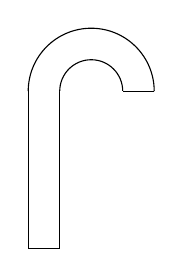
\begin{tikzpicture}[Candycane/.style = {pattern = north west line}]
        \draw[black, fill = white] (0, 2) arc (180:0:.8);
        \draw[black, fill = white] (.4, 2) arc (180:0:.4);
        \draw[black] (0, 0) -- (0, 2);
        \draw[black] (.4, 0) -- (.4, 2);
        \draw[black] (0, 0) -- (.4, 0);
        \draw[black] (1.2, 2) -- (1.6, 2);
        \draw[white] (.4, 2) -- (1.2, 2);
        \vstripe{(0,.2)}{(0, .4)}{(.4, .35)}{(.4, .15)}
        \vstripe{(0,.8)}{(0, 1)}{(.4, .95)}{(.4, .75)}
        \vstripe{(0, 1.4)}{(0, 1.6)}{(.4, 1.55)}{(.4, 1.35)}
        %\roundstripe{180}{165}{.8}{.4}{(0, 2)}

    \end{tikzpicture}
\end{center}
\end{document}